\scanpage{106}
% archive foliation: 105
% Typescript is upside down relative to archive foliation.
\begin{center}- IV- \inserted{\unsure{878}} -\end{center}

\uline{un point de} $Y$.

Il résulte en effet de (17.4.1,(b'')) qu'une $Y$-section $s$ de $X$ est une immersion ouverte, et comme $X$ est un $Y$-schéma, $s$ est aussi une \deleted{\illegible{1}} immersion fermée (\uline{I},5.4.7); il en résulte que $s$ est un isomorphisme de $Y$ sur un sous-préschéma de $X$ induit sur une partie ouverte et fermée de $X$, et comme \deleted{\unsure{$X$}} $s(Y)$ est connexe, c'est nécessairement une composante connexe de $X$. Le reste de la proposition est immédiat.

\margin{\figure{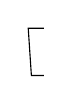
\begin{tikzpicture}\draw (0.20,0.6)--(0,0.6)--(0.04,0)--(0.2,0);\end{tikzpicture}}}
\uline{Proposition} (17.4.10) .- \uline{Soient} $g:Y\to S$, $h:X\to S$ \uline{deux morphismes localement de présentation finie. Pour qu'un} $S$-\uline{morphisme} $f:X\to Y$ \uline{soit non ramifié il faut et il suffit que pour tout} $s\in S$, \uline{le morphisme} $f_s:h^{-1}(s)\to g^{-1}(s)$ \uline{déduit de $f$ par le} \deleted{\illegible{1}} \uline{changement de base} $\operatorname{Spec}(\kappa(s))\to S$, \uline{soit non ramifié}.

Cela résulte aussitôt du fait que pour un morphisme localement de présentation finie, le fait d'être non ramifié est une propriété des \uline{fibres} de ce morphisme \inserted{(17.4.1,d))}, et \inserted{de ce} que pour tout $y\in Y$, on a $f^{-1}(y)=f_s^{-1}(y)$ si $s=g(y)$.
\margin{\figure{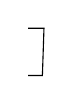
\begin{tikzpicture}\draw (0,0.6)--(0.2,0.6)--(0.18,0)--(0,0);\end{tikzpicture}}}

\uline{17.5. Caractérisations des morphismes lisses}.

\uline{Théorème} (17.5.1) .- \uline{Soient} $f:X\to Y$ \uline{un morphisme localement de présentation finie, $x$ un point de} $X$, $y=f(x)$. \uline{Les conditions suivantes sont équivalentes}:

a) \uline{$f$ est lisse au point $x$}.

\margin{\figure{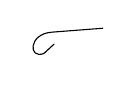
\begin{tikzpicture}[x=1cm,y=1cm]
\draw (1,.35)--(.35,.3) .. controls (.05,.28) and (.05,-.05) .. (.25,.03)--(.38,.15);
\end{tikzpicture}}}
b) \uline{$f$ est plat au point $x$ et le} $\kappa(y)$-\uline{préschéma} $f^{-1}(y)$ \uline{est lisse sur} $\kappa(y)$ \uline{au point $x$}.

b') \uline{$f$ est régulier au point $x$} (6.8.1).

c) \uline{L'anneau} $\mathrm O_{X,x}$ \uline{est une} $\mathrm O_{Y,y}$-\uline{algèbre formellement lisse pour les topologies discrètes}.

\margin{\figure{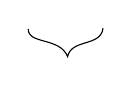
\begin{tikzpicture}[x=1cm,y=1cm]
\draw (0,.35) .. controls (0,.15) and (.4,.25) .. (.5,0) .. controls (.55,.23) and (.92,.12) .. (.95,.36);
\end{tikzpicture}}}
On peut se borner au cas où $Y=\operatorname{Spec}(A)$, \deleted{\unsure{$X=\operatorname{Spec}$}} $X=\operatorname{Spec}(C)$, où $C=B/\uline{J}$, $B=A[T_1,\ldots,T_n]$ étant une algèbre de polynômes et $\uline{J}$ un idéal de $B$ \uline{de type fini}. L'équivalence de a) et c) résulte alors de (\uline{0},22.6.4)\inserted{a)$\Leftrightarrow$c)}. D'autre part, comme $f^{-1}(y)$ est un $\kappa(y)$-préschéma localement \deleted{noethérien} \inserted{de type fini}, l'équivalence de b) et b') résulte de (6.8.6)\inserted{a)$\Leftrightarrow$b)}. Reste à voir que a) et b) sont équivalentes.

\margin{\diagram{\begin{tikzcd}[column sep=small]
{} \arrow[r,bend right] & \text{Attention à l'ambiguïté dans ``lisse'' !}
\end{tikzcd}}}
